\section{Background} 
\label{sec:bg}
In this section we give a brief overview of DRAM, covering the organization, basic operation, refresh modes, and trends together with projections for the DRAM structure.

DRAM is hierarichally organized as \reffig{fig:dram_orga} shows. At the top of the hierarchy are the channels that are connected to one or more ranks. Each channel has individual address, data, and command buses that makes it possible for the channels to operate cuncurrently. All ranks on one channel can operate in parallel constrained by the channel bandwith which is shared among the ranks. A rank comprizes of several banks where one bank holds a DRAM cell array. The banks are thus also able to work in parallel, but are constrianed by both the shared channel bandwith and resources shared among the banks. 

The DRAM cell array in each bank is structured as \reffig{fig:dram_orgb} shows. One cell consists of a transistor and a capacitor, where the transistor is controlled by the wordline wire and connects the capacitor to the bitline wire. The wordline connects a number of cells which forms a row. Each bitline is connected to a sens amplifier and the row of sens amplifier constitutes the row buffer. Data is stored as a charge on the cell capacitor.

\begin{figure*}[t]
    \centering
    \subfigure[DRAM hierarcy]{
        \centering
        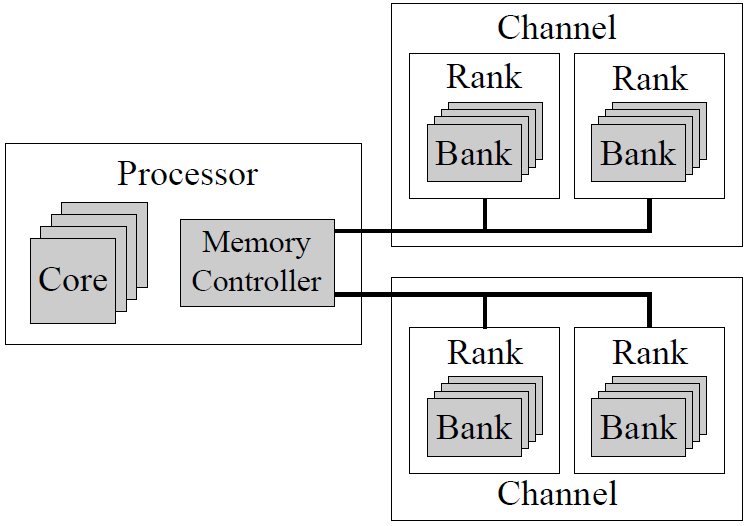
\includegraphics[width=0.4\textwidth]{dram_orga}
		\label{fig:dram_orga}
    }
    \subfigure[DRAM bank structure]{
        \centering
        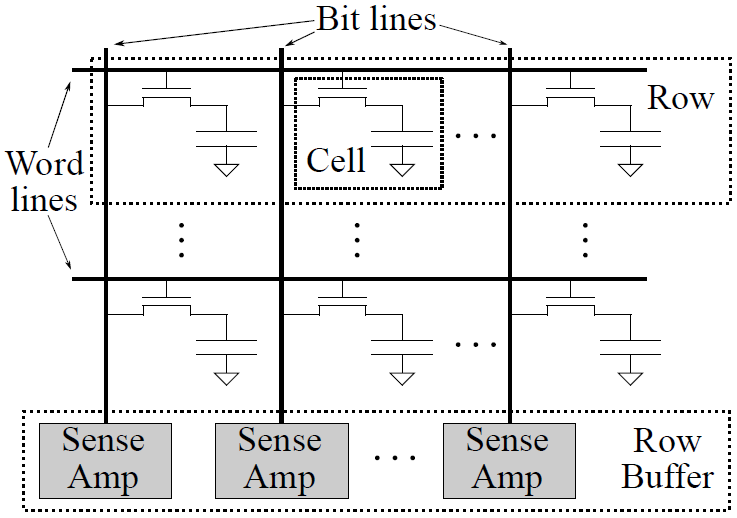
\includegraphics[width=0.4\textwidth]{dram_orgb}
		\label{fig:dram_orgb}
    }
	\caption{DRAM system organization \cite{raidr}.}
	\label{fig:dram_org}
\end{figure*}

To read or write to a DRAM cell the wordline connected to the targeted transistor must first be activated. When the wordline is activated, the transistor connects the capacitor to the bitline. For this to work, the bitlines has to be precharged to \(V_{DD}\)/2. When the capacitor connects to the bitline, charge will either flow from or to the capacitor depending on if the capacitor was charged or not, respectively. The sens amplifier will detect the change of voltage and drive the bitline either to \(V_{DD}\) or 0 V. Data can then be read from the bitline. If data is to be written the corresponding voltage is applied to the bitline, which stores the data in the capacitor. Finally, if another row on the bank chall be accessed the open row has to be closed, which disconnects the capacitors from the bitlines.

Over time the capacitors leaks charge and the capacitor has to be recharged in order to preserve the data. The operation to recharge a row is called refresh and is performed by opening a row to let the sense amplifiers amplify the detected voltage change and thus recharge the cells to either \(V_{DD}\) or 0 V. This follows the same procedure as a read operation and thus is the row refreshed when a read is performed. 

The memory controller (MC) normally issues the refresh operation, the auto-refresh command, periodically at an interval of 64 ms for each row, an interval that has been constant for the latests DRAM specifications. The interval is halved if the DRAM exeeds the specified working temprature of 85$^{\circ}$C. The average time between refresh commands are issued by the MC is denoted \(t_{REFI}\) and the time it takes to perform the refresh is denoted \(t_{RFC}\), i.e the time where no normal access requests can be serviced.

To refresh one rank, the simplest approach is to refresh all banks in parallel row-by-row at the start of the 64ms interval. This approch is called Burst refresh and has some downsides. The approch blocks normal accesses for a longer period and form a peak of power consumption during the burst time. A better alternative is to distribute the refreshes across the interval, resulting in a lower average latency for the processor and a more stable power consumption.

The implementation of a DRAM refresh cycle can be made in two different ways, to either affect one row or many. The first is called RAS-only refresh (ROR) where refresh cycle refreshes one targeted row. The address for the targeted row has to be put on the bus and it is the MC that makes sure that a row are refreshed within the 64ms interval. The second is called CAS before RAS refresh (CBR). In this scheme the memory module has an internal address counter that displays which row that shall be refreshed. On a refresh cycle, the row stated by the internal address counter is refreshed and the counter is then incremented. The advantage with this method is that the address is never put on the bus, which gives a lower power consumption and less bus usage than ROR. CBR is the most used method and is the one normally implemented in the auto-refresh command. 

When using auto-refresh (CBR), all banks in a rank are blocked for normal accesses. All banks are also blocked when ROR is used due to DRAM chip design, however some DRAM chips support per-bank refresh commands that makes it possible to only block the specific bank which is getting refreshed. 

As m

\begin{figure}[t]
    \centering
    \subfigure[DRAM throughput loss]{
        \centering
        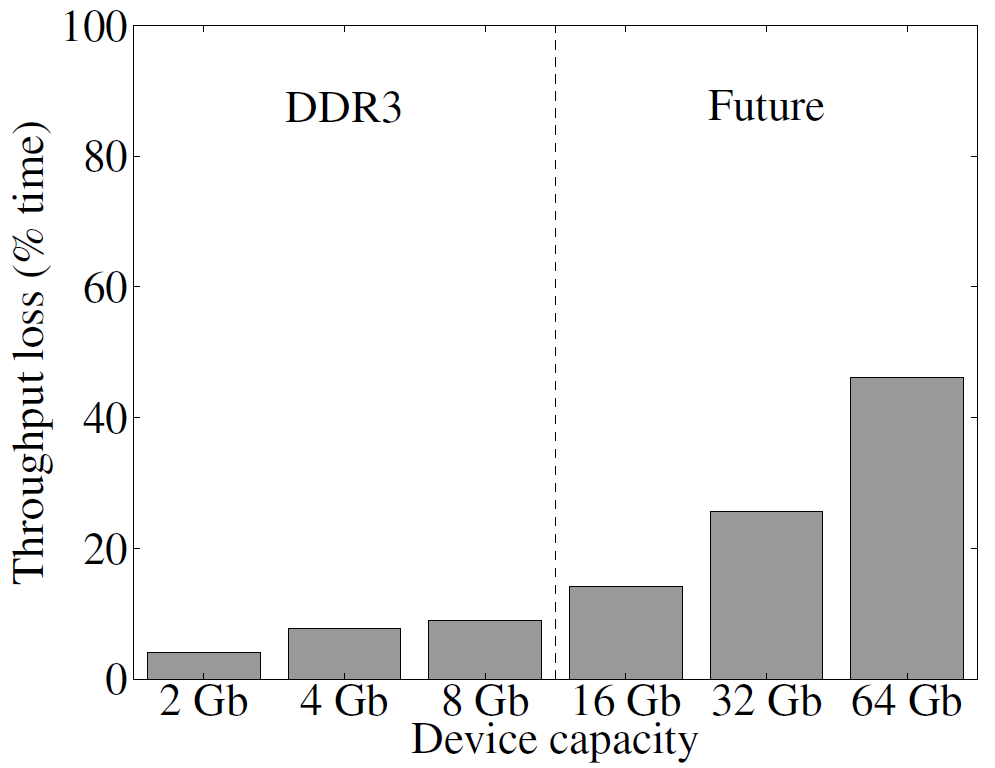
\includegraphics[width=0.33\textwidth]{dram_throughput}
        \label{fig:dram_throughput}
    }
    \subfigure[DRAM power consumption]{
        \centering
        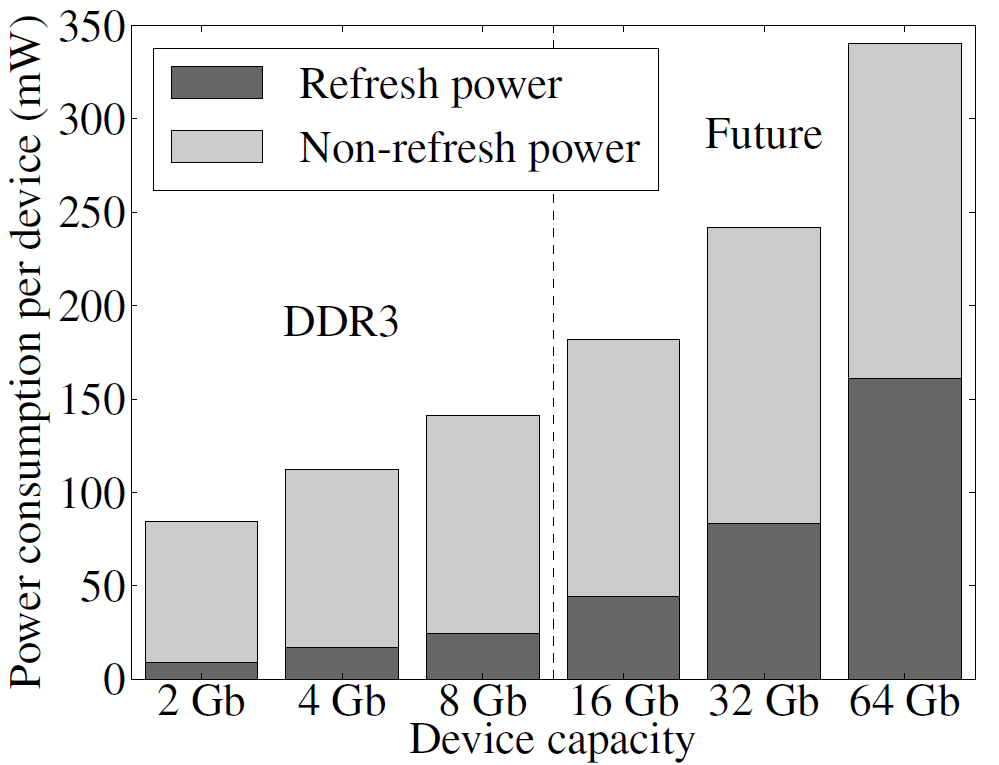
\includegraphics[width=0.33\textwidth]{dram_power}
        \label{fig:dram_power}
    }%
    \caption{Projections on DRAM throughput loss and power consumption \cite{raidr}.}
    \label{fig:dram_data_proj}
\end{figure}


Trends - Storage array rectangular
            cant go wider (word lines length = timing = power)
            gets taller = more refreshes
            over time .... projektions (see Intel)
